\documentclass[10pt]{beamer}

\usepackage[utf8]{inputenc}
\usepackage{tcolorbox}
\usepackage{tikz}
\usepackage{tikz-3dplot}
\usetikzlibrary{intersections,calc,,angles,quotes,through}
\usepackage{amsmath}
\usepackage{graphicx}
\usepackage{cases}
\def \heart {\textcolor{blue}{$\heartsuit$} }
\def \C {\mathcal{C}}
\def \orthog {\underline{\perp}}
\def\arcos{\operatorname{arcos}}
\def \deg {^{\circ}}

\newcommand{\vect}[1] {
  \overrightarrow{#1}}

\tcbset{%
	basic/.style={colframe=black,
		      colback=white,
		      top= 0mm,
		      bottom = 2mm,
		      boxsep=0mm
		      }
}
\tikzset{
    invisible/.style={opacity=0},
    visible on/.style={alt={#1{}{invisible}}},
    alt/.code args={<#1>#2#3}{%
      \alt<#1>{\pgfkeysalso{#2}}{\pgfkeysalso{#3}} % \pgfkeysalso doesn't change the path
    },
  }

    
\begin{document}  
    \beamertemplatenavigationsymbolsempty
    \setlength{\abovedisplayskip}{0pt}
    \setlength{\belowdisplayskip}{0pt}
    \frame{
	  
	  \frametitle{Q2 Juillet 2003.}
	  %\renewcommand{\theenumi}{\alph{enumi})}
	  On considère un triangle $ABC$. Par $B$, on mène une droite $d$ variable qui
	  coupe $AC$ en $D$. Déterminer l’équation cartésienne du lieu géométrique du
	  centre de gravité du triangle $ABD$.
	  \vfill
	  
	  \pause
	  
	   \begin{tcolorbox}[basic] \smallskip
	     \centering\underline{Procédé}\flushleft
	     Dans un repère, établir les coordonnées de $D$ pour trouver l'équation cartésienne.

	  \end{tcolorbox}
    }

    \frame{\begin{columns}[t]
		\column{.5\textwidth}\centering 
				  \underline{Dessin}
				  \begin{figure}[h]
				  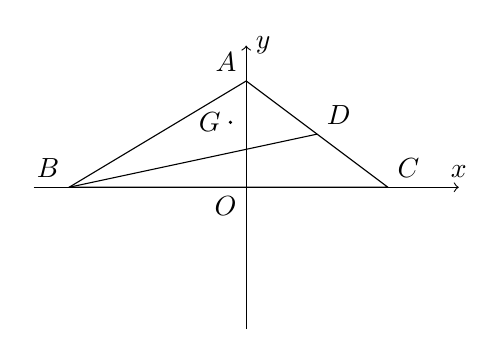
\begin{tikzpicture}[scale=0.9]
			          %projection ($(X)!(B')!(B)$)
			          %nommer chemin 'name path
			          %intersection \path [name intersections={of=d and gb,by=G}];
			          
			          %\draw[help lines] (-3,-3) grid (3,3);
			          %TRIANGLE ABC
			          \coordinate[label=below left:$O$](O) at (0,0);
			          \draw[->] (-3,0)--(3,0) node[above]{$x$};
				  \draw[->] (0,-2)--(0,2) node[right]{$y$};
				  \coordinate[label=above left:$A$] (A) at (0,1.5);
				  \coordinate[label=above left:$B$] (B) at (-2.5,0);
				  \coordinate[label=above right:$C$] (C) at (2,0);
				  \draw (A) -- (B) -- (C) -- cycle;
				  %D
				  \coordinate[label=above right:$D$] (D) at ($(A)!.5!(C)$);
				  \draw (B) -- (D);
				  \coordinate[label= left:$G$] (G) at ($(A)!.333!(B)!.333!(D)$);
				  \fill (G) circle (0.025);
				  \end{tikzpicture}
				  \end{figure}
				  
				  \begin{tcolorbox}[basic] 
				      
				    \smallskip
				    \centering\underline{Procédé} \flushleft
				    Dans un repère, établir les coordonnées de $D$ pour trouver l'équation cartésienne.
				    \end{tcolorbox}
		
		
		\column{.52\textwidth}\centering 
		 \underline{Résolution}\\ \flushleft
		 Soit un repère orthonormé $R=(O,X,Y)$ avec : \\
		 $A\ (0,a),\ B\ (b,0),\ C\ (c,0)$.\\ \bigskip
		 
		 \textit{Cas particulier : $c=0$} \\ \medskip 
		 $AC \equiv x = 0$. \\ \medskip
		 $\rightarrow D(\ 0,\ y_D). \qquad (y_D \in \mathbb{R})$ \\ \bigskip
		 $G = \frac{1}{3}A+\frac{1}{3}B+\frac{1}{3}C$. \\ \medskip
		 $G \equiv \begin{cases}
		            x=\dfrac{b}{3}, \\[0.8em]
		            y=\dfrac{a+y_D}{3}.
		           \end{cases}$ \\ \medskip
		 Lieu : $x=\frac{b}{3}$.

		%\centering\noindent\rule{2cm}{0.4pt}
		\end{columns}
    }
    
    \frame{ \begin{columns}[t]
		\column{.5\textwidth}\centering 
				  \underline{Dessin}
				  \begin{figure}[h]
				  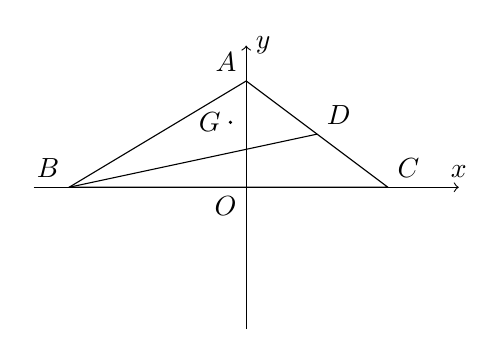
\begin{tikzpicture}[scale=0.9]
			          %projection ($(X)!(B')!(B)$)
			          %nommer chemin 'name path
			          %intersection \path [name intersections={of=d and gb,by=G}];
			          
			          %\draw[help lines] (-3,-3) grid (3,3);
			          %TRIANGLE ABC
			          \coordinate[label=below left:$O$](O) at (0,0);
			          \draw[->] (-3,0)--(3,0) node[above]{$x$};
				  \draw[->] (0,-2)--(0,2) node[right]{$y$};
				  \coordinate[label=above left:$A$] (A) at (0,1.5);
				  \coordinate[label=above left:$B$] (B) at (-2.5,0);
				  \coordinate[label=above right:$C$] (C) at (2,0);
				  \draw (A) -- (B) -- (C) -- cycle;
				  %D
				  \coordinate[label=above right:$D$] (D) at ($(A)!.5!(C)$);
				  \draw (B) -- (D);
				  \coordinate[label= left:$G$] (G) at ($(A)!.333!(B)!.333!(D)$);
				  \fill (G) circle (0.025);
				  \end{tikzpicture}
				  \end{figure}
				  
				  \begin{tcolorbox}[basic] 
				      
				    \smallskip
				    \centering\underline{Procédé} \flushleft
				    Dans un repère, établir les coordonnées de $D$ pour trouver l'équation cartésienne.
				    \end{tcolorbox}
		
		
		\column{.52\textwidth} \underline{Résolution}\\ \flushleft
		 Soit un repère orthonormé $R=(O,X,Y)$ avec : \\
		 $A\ (0,a),\ B\ (b,0),\ C\ (c,0)$.\\ \bigskip
		 
		 \textit{Cas général : $c\neq 0$} \\ \medskip 
		 $AC \equiv y=a(1-\frac{x}{c})$. \\ \medskip
		 $\rightarrow D(\ x_D,\ a(1-\frac{x_D}{c})\ ). \qquad (x_D \in \mathbb{R})$ \\ \bigskip
		 $G = \frac{1}{3}A+\frac{1}{3}B+\frac{1}{3}C$. \\ \medskip
		 \begin{numcases}{G \equiv} 
		            x=\frac{b+x_D}{3}, \\[0.2em]
		            y=\frac{a+a(1-\frac{x_D}{c})}{3}.
		           \end{numcases} \\ \medskip
		 $(1)\ x_D = 3x -b$. \\ \bigskip
		 $(2)\ \text{Lieu : } y=-\dfrac{a}{c}x + \dfrac{a}{3c}(b+2c)$.

		%\centering\noindent\rule{2cm}{0.4pt}
		\end{columns}
    }
	  
  
\end{document}
